\section{Simulation study}\label{sec:simulation}

\providecommand{\armT}{\mathsf{T}}
\providecommand{\armC}{\mathsf{C}}
\providecommand{\armD}{\mathsf{D}}
\providecommand{\SDB}{\mathrm{SDB}}

All data in this section are synthetic. Every dataset is drawn from a model whose parameters we chose, so the truth is known. No survey responses are used, and nothing here is a finding about the attitudes of any population. Every number is taken from \texttt{results/sim\_results.json}, which \texttt{code/run\_experiments.py} writes. \Cref{app:simdetails} gives the design table (\cref{tab:sim-design}), configurations, seeds, run times, code hashes, Monte Carlo standard errors (MCSE) and further results. We label the experiments X1 to X9. The first five were called E1 to E5 in an earlier version; we renamed them because those labels collided with the estimands (E1)--(E9) of the plan (\cref{sec:design-estimands}). Their seeds and results are unchanged.

\subsection{Design and estimation}\label{sec:sim-design}

X1 tests identification and recovery (\cref{thm:ident,prop:model-sl,prop:id-boundary-test}) and X9 the heterogeneity test of rule D2(ii). X2 tests DIF and anchors (\cref{thm:dif-bias,prop:anchor}), X2b DIF on the stereotype anchors (\cref{prop:anchor}(c), \cref{rem:id-anchor-S}) and X7 the revised DIF screen of the plan. X6 adds two misspecifications that the plan must guard against. X3 tests list experiments (\cref{prop:list-var,thm:joint-sdb,thm:design}) and X8 the identification of the threshold shift (\cref{prop:list-irt}). X4 tests small-area estimation (\cref{eq:mrp,prop:eap}) and X5 count indices (\cref{prop:index,prop:index-dif}). X1, X2, X2b and X7 generate data from the normal-ogive bifactor graded response model of \cref{sec:model} with five categories. The eight stereotype items have item-level ECVs between $0.45$ and $0.90$ and communalities between $0.50$ and $0.60$, so the stereotype domain satisfies \cref{asm:id-het}. The Israel-related items I1, \dots, I6 have ECVs $0.25$, $0.75$, $0.40$, $0.60$, $0.15$ and $0.85$ and communality $0.5$; a design with $|\mathcal I|$ items uses the first $|\mathcal I|$. With $\tau=0.5$ the true boundary set is $\{\mathrm{I}2\}$ for $|\mathcal I|\in\{2,3\}$ and $\{\mathrm{I}2,\mathrm{I}4,\mathrm{I}6\}$ for $|\mathcal I|=6$. X6 and X9 use the registered sizes of \cref{tab:design-items}: 10 stereotype items, 8 ID items, 6 IT items and $n=6{,}000$.

\paragraph{Estimation}
All fits use the limited-information estimator that the plan adopts as primary (\cref{sec:design-decisions}). Thresholds and polychoric correlations are estimated in two steps \citep{olsson1979}, with an asymptotic covariance matrix $\bm\Gamma$ from per-respondent influence functions. The bifactor model is fitted by weighted least squares with the diagonal weights $\operatorname{diag}(\bm\Gamma)^{-1}$, with sandwich standard errors, from a default start and random starts. For each $\mathrm{ECV}_j$ we form a logit-scale Wald interval with the sandwich standard error, and in X1 also a percentile bootstrap interval from $B=100$ resamples. Under the normal-ogive model this estimator targets the same parameters as maximum likelihood (\cref{lem:id-reduction}), but its finite-sample behaviour can differ (\cref{sec:sim-limits}).

\subsection{Recovery and identification (X1, X9)}\label{sec:sim-recovery}

X1 compares five designs with $n\in\{500,1000,3000\}$. The designs with $|\mathcal I|=6$ and $|\mathcal I|=3$ are identified by \cref{thm:ident}(a). The design with $|\mathcal I|=2$ is the case of \cref{thm:ident}(c): its two ECVs, $0.25$ and $0.75$, have the identified sets $(0.125,0.625)$ and $(0.375,0.875)$ of \eqref{eq:id-two}, and both contain $\tau$. In the \emph{proportional} design every stereotype item has ECV $0.70$ and $|\mathcal I|=3$, so \cref{thm:ident}(b) applies. The \emph{near-proportional} design has stereotype ECVs between $0.65$ and $0.75$ and $|\mathcal I|=3$; it is identified, but weakly (\cref{rem:id-heterogeneity}). The \emph{identification diagnostic} is the ratio of the smallest to the largest singular value of the weighted Jacobian of the fitted correlations, zero when the model is not locally identified. At the population values it is $0.094$ and $0.068$ in the identified designs, $0.0060$ in the near-proportional design and zero to machine precision in the other two. \Cref{tab:sim-main,fig:sim-recovery} give the results. With $R=40$, as in the proportional and near-proportional designs, the MCSE of a coverage or a classification rate is about 7 percentage points ($4.7$ to $7.9$ for the item-level and set coverages), so differences of less than about 15 points between those cells are not resolved.

\begin{table}[tbp]
\centering
\caption{X1, recovery of the boundary estimands (synthetic data; $R=100$ for $|\mathcal I|=6,3$, $50$ for $|\mathcal I|=2$, $40$ otherwise, where the MCSE of a coverage is about 7 points). Bias and RMSE of $\widehat{\mathrm{ECV}}_j$ are pooled over $j\in\mathcal I$. Cov.\ B and Cov.\ W: coverage (\%) of nominal 95\% percentile-bootstrap ($B=100$) and Wald intervals (logit scale, sandwich standard errors). Corr., Undet., Wrong: per-item classification (\%) as in, out or undetermined from the bootstrap interval, against the true $\mathcal B_{0.5}$. Set: probability (\%) that $\widehat{\mathcal B}{}^{\mathrm{in}}_{0.5}\subseteq\mathcal B_{0.5}\subseteq\widehat{\mathcal B}{}^{\mathrm{out}}_{0.5}$ with Bonferroni-adjusted Wald intervals (\cref{prop:id-boundary-test}(b)). $\hat\rho_{SI}$: correlated-factors estimate against its pseudo-true value; Cov.: sandwich interval. $^\dagger$Not identified (\cref{thm:ident}(b),(c)); the entries describe the optimiser, not the estimand.}
\label{tab:sim-main}
\footnotesize
\setlength{\tabcolsep}{4.2pt}
% Generated by code/make_figures.py from results/sim_results.json -- do not edit by hand.
% E1. Bias/RMSE pooled over the Israel-related items; Cov. B = bootstrap percentile, Cov. W = sandwich
% (logit-scale Wald) coverage of nominal 95% intervals; boundary classification from the bootstrap
% interval (in / out / undetermined vs the true ECV_j >= 0.5). R per design = {'I6': 100, 'I3': 100, 'I2': 50, 'I3p': 40, 'I3np': 40}; B = 100.
% Set: Pr(B_in subset B_tau subset B_out) with Bonferroni logit-Wald intervals (prop:id-boundary-test(b)).
% rho_SI: correlated-factors S-I correlation vs its pseudo-true value; Cov. = sandwich interval.
% dagger = not identified (thm:ident).
\begin{tabular}{@{}llrrrrrrrrrr@{}}
\toprule
 & & \multicolumn{4}{c}{$\widehat{\mathrm{ECV}}_j$, $j\in\mathcal{I}$} & \multicolumn{4}{c}{Boundary set $\mathcal{B}_{0.5}$ (\%)} & \multicolumn{2}{c}{$\hat\rho_{SI}$} \\
\cmidrule(lr){3-6} \cmidrule(lr){7-10} \cmidrule(lr){11-12}
Design & $n$ & Bias & RMSE & Cov.\ B & Cov.\ W & Corr. & Undet. & Wrong & Set & RMSE & Cov. \\
\midrule
$|\mathcal{I}|=6$ & 500 & +0.005 & 0.082 & 95 & 95 & 66 & 34 & 0 & 100 & 0.034 & 96 \\
 & 1000 & +0.006 & 0.062 & 91 & 93 & 73 & 27 & 0 & 100 & 0.028 & 94 \\
 & 3000 & +0.004 & 0.035 & 92 & 96 & 91 & 9 & 0 & 100 & 0.016 & 94 \\
\addlinespace
$|\mathcal{I}|=3$ & 500 & +0.038 & 0.141 & 95 & 94 & 39 & 61 & 0 & 98 & 0.042 & 97 \\
 & 1000 & +0.002 & 0.074 & 97 & 96 & 57 & 43 & 0 & 100 & 0.030 & 96 \\
 & 3000 & +0.004 & 0.046 & 95 & 96 & 77 & 23 & 0 & 100 & 0.019 & 95 \\
\addlinespace
$|\mathcal{I}|=3$, near-prop.\ $S$ & 500 & $-$0.005 & 0.202 & 92 & 73 & 38 & 62 & 0 & 88 & 0.044 & 90 \\
 & 1000 & +0.020 & 0.192 & 92 & 57 & 48 & 52 & 0 & 72 & 0.034 & 92 \\
 & 3000 & +0.023 & 0.168 & 88 & 58 & 63 & 35 & 2 & 72 & 0.021 & 90 \\
\addlinespace
$|\mathcal{I}|=2$$^{\dagger}$ & 500 & +0.032 & 0.177 & 89 & 81 & 45 & 55 & 0 & 98 & 0.060 & 96 \\
 & 1000 & +0.021 & 0.105 & 89 & 86 & 73 & 27 & 0 & 100 & 0.035 & 94 \\
 & 3000 & +0.001 & 0.106 & 65 & 62 & 88 & 12 & 0 & 98 & 0.028 & 90 \\
\addlinespace
$|\mathcal{I}|=3$, prop.\ $S^{\dagger}$ & 500 & $-$0.037 & 0.182 & 91 & 71 & 44 & 56 & 0 & 90 & 0.044 & 95 \\
 & 1000 & $-$0.050 & 0.180 & 91 & 54 & 40 & 59 & 1 & 88 & 0.028 & 98 \\
 & 3000 & $-$0.047 & 0.168 & 60 & 25 & 70 & 28 & 2 & 82 & 0.017 & 95 \\
\bottomrule
\end{tabular}

\end{table}

\paragraph{Identified designs}
With $|\mathcal I|=6$ the pooled bias of $\widehat{\mathrm{ECV}}_j$ is at most $0.006$ and the RMSE falls from $0.082$ to $0.035$ as $n$ grows from 500 to 3{,}000. With $|\mathcal I|=3$ the RMSE is $0.141$, $0.074$ and $0.046$; the bias of $+0.038$ at $n=500$ comes with fits at a slope bound in 6\% of replications. Wald intervals cover in $93.2$ to $96.3\%$ of cases and bootstrap intervals in $91.0$ to $97.0\%$. No item is classified on the wrong side of $\tau$, except in $0.2\%$ of cases for $|\mathcal I|=6$ at $n=500$, and the share classified correctly rises from $66.2\%$ to $91.0\%$ with $|\mathcal I|=6$ and from $39.0\%$ to $77.0\%$ with $|\mathcal I|=3$. Items near $\tau$ stay undetermined longest: at $n=3{,}000$ with $|\mathcal I|=6$, I3 (ECV $0.40$) and I4 ($0.60$) are classified correctly in $67\%$ and $79\%$ of replications and every other item in $100\%$. Comparing point estimates with $\tau$ instead would misclassify $5.2\%$, $2.7\%$ and $0.2\%$ of the items, with no indication of which (\cref{prop:id-boundary-test}(c)). With Bonferroni-adjusted Wald intervals, the rule of the plan, the inner and outer sets bracket $\mathcal B_{0.5}$ in $100\%$ of replications with $|\mathcal I|=6$ and in $98$ to $100\%$ with $|\mathcal I|=3$ (column Set), at the price of more undetermined items ($43.2\%$, $65.0\%$ and $82.3\%$ correct with $|\mathcal I|=6$).

\begin{figure}[tbp]
\centering
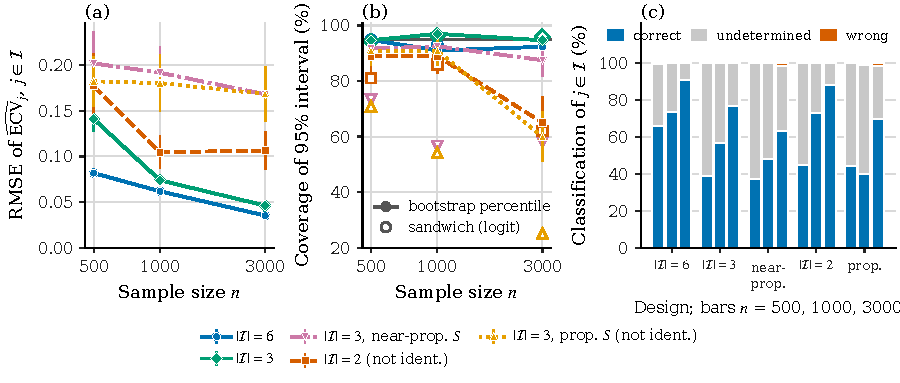
\includegraphics[width=6.0in]{figures/fig-sim-recovery.pdf}
\caption{X1, recovery of the item-level ECV and of the boundary set $\mathcal B_{0.5}$ (synthetic data). (a) RMSE of $\widehat{\mathrm{ECV}}_j$, pooled over the Israel-related items ($\pm2$ MCSE bars). (b) Coverage of nominal 95\% intervals: percentile bootstrap with $B=100$ (filled markers) and Wald intervals on the logit scale with sandwich standard errors (open markers, ``Wald (sandwich)''). (c) Classification of each Israel-related item from its bootstrap interval, against the true boundary set; bars are $n=500$, $1{,}000$ and $3{,}000$. The designs in grey are not identified ($|\mathcal I|=2$ and proportional $S$; \cref{thm:ident}(b),(c)) or only weakly identified (near-proportional $S$). Their ``correct'' shares, up to $88\%$, describe where the optimiser stops, not information in the data.}
\label{fig:sim-recovery}
\end{figure}

\paragraph{Non-identified and weakly identified designs}
With $|\mathcal I|=2$ the diagnostic is below $0.01$ in every replication, and the five starts reach the same objective value, within a relative $10^{-6}$, at points whose ECVs differ by $0.19$ to $0.22$ on average. The reported estimate is whichever point wins on rounding error, so its ``correct'' classifications carry no information from the data: both identified sets contain $\tau$, and bootstrap coverage falls from $89\%$ to $65\%$ as $n$ grows. In the proportional design sampling noise tilts the flat population objective, all starts reach the same point and the optimiser reports convergence in $92.5$ to $97.5\%$ of replications, yet the ECVs are not identified. The diagnostic is small (median $0.028$, $0.027$ and $0.0013$, against $0.061$ to $0.101$ in the identified designs), $35$ to $47.5\%$ of fits put a slope at its bound, the RMSE stays near $0.17$ to $0.18$, and Wald coverage falls from $71\%$ to $25\%$. The near-proportional design degrades continuously, as \cref{rem:id-heterogeneity} predicts. Its starts agree, but the median diagnostic is $0.012$ to $0.016$, its RMSE is $0.202$, $0.192$ and $0.168$ (against $0.141$, $0.074$ and $0.046$ for the identified design with the same Israel-related items), Wald coverage is $57$ to $73\%$ and $1.7\%$ of items are misclassified at $n=3{,}000$. The estimates wander along the near-flat curve from sample to sample, not from start to start. Agreement across starts therefore exposed the two-item case but neither the proportional nor the near-proportional case; the identification diagnostic flagged all three. The correlated-factors $\hat\rho_{SI}$ is recovered against its pseudo-true value ($0.589$ to $0.621$) in every design, including the non-identified ones (RMSE $0.016$ to $0.060$, coverage $90$ to $97.5\%$), so a precise $\hat\rho_{SI}$ says nothing about the boundary (\cref{thm:ident}(d)).

\paragraph{Testing heterogeneity (X9)}
Rule D2(ii) asks the data whether \cref{asm:id-het} holds before any ECV is reported. By \cref{lem:app-tetrad,lem:app-classes}, the assumption fails in a domain $\mathcal D$ exactly when every polychoric tetrad among its items vanishes. Its failure is therefore the null hypothesis of a single \emph{joint test}, the Wald test of a non-redundant set of $|\mathcal D|(|\mathcal D|-3)/2$ tetrads (35 for the stereotype domain, 77 for the Israel-related one; \cref{app:sim-est}). X9 compares it with the \emph{intersection--union test}, which accepts heterogeneity only if the joint test of $\mathcal D\setminus\{k\}$ rejects for every $k\in\mathcal D$, and with the \emph{earlier rule}, one of the $3{,}633$ within-domain tetrads significant after a Bonferroni adjustment (\cref{tab:sim-tetrad}). At $n=6{,}000$ the joint test has size $5.0$ to $6.5\%$ in each domain under both null configurations, the rule built on it (either domain, each at $2.5\%$) rejects in $5.2$ to $5.8\%$, and it rejects in every replication in the heterogeneous and two-lines configurations. At $n=1{,}500$ it over-rejects in the Israel-related domain ($11.0$ and $14.5\%$), so at smaller samples it should be calibrated by simulation. The intersection--union test is valid but very conservative (size at most $2.5\%$), because all its component hypotheses are true whenever \cref{asm:id-het} fails. It also tests a stronger property, heterogeneity that survives the removal of any one item: when heterogeneity rests on two items on a second line, it rejects in only $3.0$ and $3.5\%$ of replications at $n=6{,}000$, against $100\%$ for the joint test. The earlier rule is not powerless at the registered sizes ($100\%$ in the heterogeneous and two-lines configurations at $n=6{,}000$), but in the stereotype domain at $n=1{,}500$ its power is $52.0\%$ against $82.5\%$ for the joint test. No test detects the near-proportional configuration (rejection rates $6.2$ to $8.0\%$ at $n=6{,}000$); there the guard is the diagnostic of rule D2(iii).

\begin{table}[tbp]
\centering
\caption{X9, tests of within-domain heterogeneity (\cref{asm:id-het}) at the registered sizes (synthetic data; $R=400$ at $n=6{,}000$, $200$ at $n=1{,}500$). Rejection rates (\%) per domain at the 5\% level of the joint tetrad test, the intersection--union test (IUT) and the earlier Bonferroni rule over $3{,}633$ tetrads; D2(ii): heterogeneity accepted in at least one domain, with the joint and intersection--union tests at $2.5\%$ per domain. $^{0}$\Cref{asm:id-het} fails in both domains, so the rates are sizes. Two lines: two items of each domain lie on a second line through the origin of the loading plane.}
\label{tab:sim-tetrad}
\footnotesize
\setlength{\tabcolsep}{3.6pt}
% Generated by code/make_figures.py from results/sim_results.json -- do not edit by hand.
% X9: rejection rates (%) of tests of within-domain heterogeneity; R = {'6000': 400, '1500': 200}. Joint: Wald test of a
% non-redundant set of |D|(|D|-3)/2 tetrads at 5%; IUT: intersection-union test (joint test of every D minus
% one item rejects at 5%); Earlier: any of the 3633 within-domain tetrads, Bonferroni at 5%. D2(ii) columns: joint and IUT at 2.5% per domain; earlier rule as stated.
% superscript 0: configurations in which id-het fails (null); rejection rates there are sizes.
\begin{tabular}{@{}lrrrrrrrrrr@{}}
\toprule
 & & \multicolumn{3}{c}{Stereotype domain ($|\mathcal S|=10$)} & \multicolumn{3}{c}{Israel domain ($|\mathcal I|=14$)} & \multicolumn{3}{c}{D2(ii): either domain} \\
\cmidrule(lr){3-5} \cmidrule(lr){6-8} \cmidrule(lr){9-11}
Configuration & $n$ & Joint & IUT & Earlier & Joint & IUT & Earlier & Joint & IUT & Earlier \\
\midrule
Proportional$^{0}$ & 1500 & 9.0 & 0.5 & 0.5 & 11.0 & 1.0 & 4.0 & 13.0 & 0.0 & 4.5 \\
 & 6000 & 5.0 & 0.0 & 0.8 & 6.0 & 0.2 & 4.2 & 5.8 & 0.2 & 5.0 \\
\addlinespace
All but one proportional$^{0}$ & 1500 & 8.0 & 0.0 & 0.0 & 14.5 & 2.5 & 2.0 & 12.5 & 1.5 & 2.0 \\
 & 6000 & 5.5 & 0.0 & 0.5 & 6.5 & 1.0 & 4.8 & 5.2 & 0.5 & 5.0 \\
\addlinespace
Two lines & 1500 & 69.5 & 4.5 & 68.5 & 54.0 & 2.5 & 70.0 & 75.0 & 4.0 & 92.5 \\
 & 6000 & 100.0 & 3.0 & 100.0 & 100.0 & 3.5 & 100.0 & 100.0 & 3.2 & 100.0 \\
\addlinespace
Near-proportional & 1500 & 12.0 & 0.0 & 2.0 & 14.0 & 1.5 & 5.0 & 13.0 & 0.5 & 7.0 \\
 & 6000 & 8.0 & 0.2 & 1.0 & 6.2 & 0.5 & 4.0 & 7.0 & 0.0 & 5.0 \\
\addlinespace
Heterogeneous & 1500 & 82.5 & 30.0 & 52.0 & 100.0 & 99.5 & 100.0 & 100.0 & 100.0 & 100.0 \\
 & 6000 & 100.0 & 100.0 & 100.0 & 100.0 & 100.0 & 100.0 & 100.0 & 100.0 & 100.0 \\
\bottomrule
\end{tabular}

\end{table}

\subsection{Differential item functioning and anchors (X2, X2b, X7)}\label{sec:sim-dif}

X2 uses the six-item design in a reference and a focal group of $1{,}500$ each, with focal latent means $(\mu_G,\mu_S,\mu_I)=(0.3,0,0.3)$. In the focal group, I1 and I2 have uniform DIF, with thresholds lowered by $\kappa$ standard deviations of the latent response, and I3 has non-uniform DIF, with its general slope multiplied by $1-1.25\kappa$; its focal ECV falls from $0.40$ to $0.273$, $0.143$ and $0.040$ at $\kappa=0.2$, $0.4$ and $0.6$. \emph{Ignore DIF} fits the invariant model to both groups (\cref{rem:id-concurrent}); the \emph{oracle} frees exactly the DIF items; the \emph{anchored} fits hold an anchor set invariant and free all other items, with the correct set S1--S4, I5, I6 or one or two contaminated anchors (I1 for I5; I1, I2 for I5, I6). The \emph{drafted screen} adds a Wald test of equal slopes and thresholds for each non-anchor item, Benjamini--Hochberg at $q=0.05$, a flag only if the expected item scores also differ by at least $0.25$ at the focal mean of $G$, and a refit with flagged items free. The \emph{revised screen} of the plan (\cref{sec:design-groups}) drops the effect-size requirement; X7 runs it end to end on the same 400 data sets. \emph{Stereotype-only anchors} use S1--S4 and fix the focal $\mu_I$ and $\sigma^2_I$ (\cref{rem:id-anchor-S}). \Cref{tab:sim-dif} gives the results at $\kappa=0.4$; \cref{fig:sim-dif,tab:sim-difrev} in \cref{app:sim-tables} give them across $\kappa$.

\begin{table}[tbp]
\centering
\caption{X2 and X7, group comparisons under DIF at $\kappa=0.4$ (synthetic data; $1{,}500$ per group; $R=100$, the same data sets in every row). Bias, RMSE and coverage (\%, sandwich 95\% interval) of the focal-minus-reference latent mean differences, and bias of the reference and focal ECV of I3, the item with non-uniform DIF (true values $0.40$ and $0.143$). Drafted screen: Benjamini--Hochberg and an expected-score difference of at least $0.25$ (X2); revised screen: Benjamini--Hochberg alone, the rule of the plan (X7).}
\label{tab:sim-dif}
\footnotesize
\setlength{\tabcolsep}{4.0pt}
% Generated by code/make_figures.py from results/sim_results.json -- do not edit by hand.
% E2 at kappa = 0.4; n = 1500 per group; R = 100. Cov.: sandwich 95% interval.
% ECV_I3: the non-uniform-DIF item, true ECV 0.40 (reference) and 0.143 (focal).
\begin{tabular}{@{}lrrrrrrrr@{}}
\toprule
 & \multicolumn{3}{c}{$\mu_G^{(1)}-\mu_G^{(0)}=0.3$} & \multicolumn{3}{c}{$\mu_I^{(1)}-\mu_I^{(0)}=0.3$} & \multicolumn{2}{c}{$\mathrm{ECV}_{I3}$ bias} \\
\cmidrule(lr){2-4} \cmidrule(lr){5-7} \cmidrule(lr){8-9}
Strategy & Bias & RMSE & Cov. & Bias & RMSE & Cov. & Ref. & Focal \\
\midrule
Ignore DIF (full invariance) & +0.036 & 0.074 & 82 & +0.243 & 0.255 & 3 & $-$0.072 & +0.199 \\
Oracle (true DIF items free) & $-$0.006 & 0.047 & 98 & +0.008 & 0.062 & 95 & +0.009 & $-$0.002 \\
Correct anchors, free baseline & $-$0.008 & 0.049 & 100 & +0.010 & 0.065 & 95 & +0.010 & $-$0.002 \\
Correct anchors, tested + refit & +0.007 & 0.046 & 98 & $-$0.032 & 0.064 & 94 & $-$0.109 & +0.146 \\
1 contaminated anchor & $-$0.170 & 0.179 & 22 & +0.744 & 0.751 & 0 & +0.047 & +0.014 \\
1 contaminated, tested + refit & $-$0.117 & 0.129 & 48 & +0.688 & 0.696 & 0 & +0.058 & +0.021 \\
2 contaminated anchors & +0.149 & 0.191 & 54 & +0.669 & 0.682 & 0 & +0.003 & $-$0.005 \\
2 contaminated, tested + refit & +0.054 & 0.101 & 82 & +0.753 & 0.760 & 0 & $-$0.008 & $-$0.010 \\
Stereotype-only anchors (S1-S4) & $-$0.011 & 0.069 & 97 & \multicolumn{3}{c}{not identified} & +0.014 & $-$0.003 \\
\bottomrule
\end{tabular}

\end{table}

\paragraph{Ignoring DIF and anchors}
DIF confined to the Israel-related items is absorbed mainly by $\mu_I$, whose bias is $+0.098$, $+0.243$ and $+0.756$ at the three non-zero values of $\kappa$. It leaks into $\mu_G$ much less ($+0.029$, $+0.036$, $-0.001$), consistent with \cref{thm:dif-bias}(d)(ii). The ECVs move more: the focal ECV of I3 is overstated by $0.091$, $0.199$ and $0.381$, and at $\kappa=0.4$ the focal ECVs of the DIF-free items I4, I5 and I6 move by $+0.055$, $+0.044$ and $+0.030$, as \cref{thm:dif-bias}(d)(iii) predicts. With the correct anchors, and for the oracle, the bias of both mean differences and of both ECVs of I3 is at most $0.010$ in absolute value, and coverage is $92$ to $100\%$. One contaminated anchor biases $\hat\mu_G$ by $-0.093$, $-0.170$ and $-0.222$, with coverage falling to $3\%$; two bias it by $+0.083$, $+0.149$ and $+0.227$. The error does not stay with the faulty anchor (\cref{prop:anchor}): the screen flags DIF-free items at rates of $29.8\%$ and $42.9\%$ at $\kappa=0.4$, against $0.0\%$ with the correct anchors. The leave-one-anchor-out range of $\hat\mu_G$ is $0.043$ with the correct anchors and $0.133$ and $0.099$ with one and two contaminated ones. Stereotype-only anchors give $\hat\mu_G$ with bias between $-0.011$ and $0.000$ and coverage $94$ to $97\%$, at the cost of a larger RMSE ($0.069$ to $0.082$, against $0.049$ to $0.061$). In X2 that protection holds by construction, because only Israel-related items have DIF; X2b removes that feature.

\paragraph{The DIF screen, drafted and revised (X7)}
With the correct anchors the drafted screen never flags a DIF-free item, but it flags I3 in $0\%$, $0\%$ and $1\%$ of replications at $\kappa=0.2$, $0.4$ and $0.6$: a change in the general slope alone barely moves the expected score at the focal mean. It then treats I3 as invariant and reproduces the bias it is meant to prevent: at $\kappa=0.4$ the ECV of I3 is biased by $-0.109$ in the reference group and $+0.146$ in the focal group. We therefore revised the plan so that the multiplicity-adjusted test alone decides which items are freed, and re-simulated the revised screen end to end (X7). Its flags coincide with the Benjamini--Hochberg flags of X2 in every replication. With the correct anchors it frees I1 and I2 in $94$ and $98\%$ of replications at $\kappa=0.2$ and in $100\%$ at $\kappa\ge0.4$, and I3 in $41\%$, $100\%$ and $100\%$. It flags DIF-free items at mean rates of $0.7\%$, $3.6\%$, $2.8\%$ and $1.6\%$ at $\kappa=0$, $0.2$, $0.4$ and $0.6$, which costs precision but not bias. Downstream, $\hat\mu_G$ has bias between $-0.006$ and $0.000$ and coverage $95$ to $98\%$ at every $\kappa$, and the focal ECV of I3 is biased by $+0.042$, $-0.002$ and $+0.002$, against $+0.082$, $+0.146$ and $+0.190$ for the drafted screen. The remaining bias at $\kappa=0.2$ comes from the $59\%$ of replications in which I3 is not flagged ($+0.077$ there): small non-uniform DIF stays hard to detect with $1{,}500$ per group. With contaminated anchors the revised screen does not help ($\hat\mu_G$ biased by $-0.123$ and $+0.070$ at $\kappa=0.4$); only the choice of anchors addresses that.

\paragraph{DIF on the stereotype anchors (X2b)}
X2b gives two of the four stereotype anchors, S1 and S2, uniform DIF of $\kappa_S\in\{0.1,0.2,0.3\}$ in the same direction, with or without the Israel-related DIF of X2 at $\kappa_I=0.4$ (\cref{tab:sim-anchors}). At $\kappa_S=0.1$ the mean bias of $\hat\mu_G$ is $+0.025$ and $+0.031$ with the default anchors S1--S4, I5, I6 (coverage $96$ and $89\%$) and $+0.073$ and $+0.080$ with stereotype-only anchors (coverage $84$ and $75\%$). At $\kappa_S=0.2$ it is $+0.047$ and $+0.069$ against $+0.259$ and $+0.410$ (probability limits of the latter $+0.254$ and $+0.266$), and at $\kappa_S=0.3$ the stereotype-only fit breaks down (probability limits $+2.521$ and $+2.634$) while $21$ to $22\%$ of the default fits fail to converge. Stereotype-only anchoring is therefore not a safe default. It drops the assumption that Israel-related anchors are invariant at the price of resting everything on four stereotype items, and the same DIF on those items biases $\hat\mu_G$ two to three times as much as with the six default anchors (to first order, $+0.058$ against $+0.026$ per $0.1$ of $\kappa_S$), and more than linearly as $\kappa_S$ grows. The contamination leaves traces: at $\kappa_S=0.1$ and $\kappa_I=0$ the leave-one-anchor-out range of $\hat\mu_G$ is $0.165$ (default) and $0.464$ (stereotype-only), against $0.043$ with clean anchors, and the revised screen flags DIF-free stereotype items in up to $11\%$ of replications ($57\%$ at $\kappa_S=0.2$), which also reduces the bias of the default-anchor comparison to $+0.006$ and $+0.013$. The bound \eqref{eq:id-anchor-bound}, evaluated for this estimator at a stated maximum DIF $\delta$ on every anchor (\cref{app:sim-est}), is valid but wide. At $\delta=0.1$ the largest first-order bias of $\hat\mu_G$ is $0.345$ with the default anchors and $0.442$ with stereotype-only anchors, more than the true difference of $0.3$, and the norm bound is $0.707$ and $0.763$; at $\delta=0.2$, the value the plan registers, all of these double. The worst case has anchor DIF of opposite signs on anchors with different ECVs, which the model reads as a shift of $G$ against $S$; if all anchors' DIF has the same sign, the first-order bias of $\hat\mu_G$ is $0.104$ and $0.099$ at $\delta=0.1$. The pattern of X2b lies well inside the bound ($+0.026$ and $+0.058$ to first order at $\kappa_S=0.1$), but for stereotype-only anchors the probability limit exceeds the first-order value from $\kappa_S=0.2$ on, so the linear bound is not conservative there.

\subsection{Cross-loadings and acquiescence (X6)}\label{sec:sim-misspec}

X6 adds two misspecifications at the registered sizes, with 8 ID items with ECVs from $0.10$ to $0.70$ and 6 trope-based IT items with ECVs from $0.35$ to $0.85$ (\cref{app:sim-config}). In (a) every IT item also loads on $S$ with standardised loading $c\in\{0.1,0.2,0.3\}$. In (b) an acquiescence factor adds a slope $+\alpha$ to every positively worded item and $-\alpha$ to every reverse-keyed item, $\alpha\in\{0.25,0.40,0.55\}$ (standardised loadings $0.16$ to $0.36$), with the registered keying (four reverse-keyed items, two in S and two in ID, none in IT) or balanced keying (half of every block). The true values are the content ECVs of each item's own domain. Besides the standard bifactor fit we evaluate five remedies: a model with free loadings of all IT items on $S$; a method factor with one free slope and the instrument's keying, the random-intercept model of \citet{maydeuolivares2006}; a refit with $\mathcal I$ the ID items alone; the two-stage rule that the plan registers (\cref{sec:design-decisions}), which tests the mean residual correlation between IT and S items and, if the test rejects, uses the model with cross-loadings; and a one-item check proposed in an earlier draft, which tests the 60 residual correlations between IT and S items and fits a cross-loading for each IT item in turn. \Cref{fig:sim-misspec} shows the main results and \cref{tab:sim-misspec} gives them in full. Without misspecification no estimator has a bias above $0.006$ and all cover in $94$ to $95\%$ of cases.

\begin{figure}[tbp]
\centering
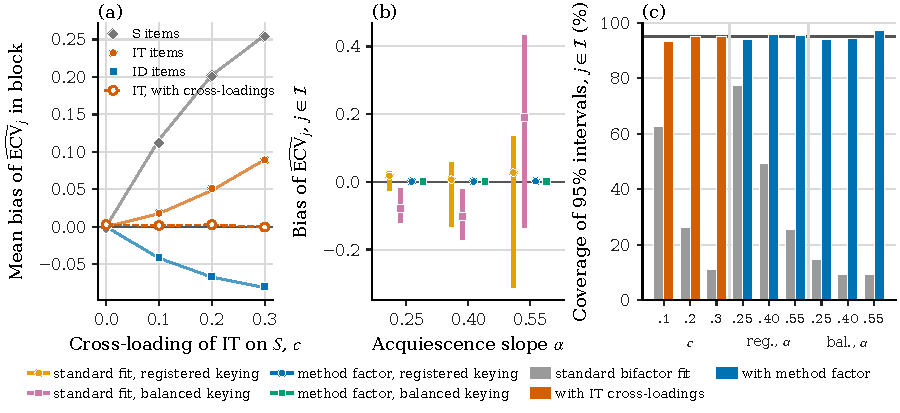
\includegraphics[width=6.0in]{figures/fig-sim-misspec.pdf}
\caption{X6, two misspecifications at the registered sizes (synthetic data; 10 S, 8 ID and 6 IT items; $n=6{,}000$; $R=100$ per cell). (a) Cross-loading of the IT items on $S$ with standardised loading $c$: mean bias of $\widehat{\mathrm{ECV}}_j$ by block in the standard bifactor fit (filled markers; lines are probability limits) and for the IT items in the model with cross-loadings (open markers). (b) Acquiescence with slope $\alpha$ and the registered (4 reverse-keyed items) or balanced keying: range (bar) and mean (marker) over the 14 Israel-related items of the bias of $\widehat{\mathrm{ECV}}_j$, in the standard fit and with a one-parameter method factor. (c) Coverage of the 95\% Wald intervals for the Israel-related ECVs in the standard fit (grey) and with the remedy for each misspecification: cross-loadings in the first three cells, the method factor in the others.}
\label{fig:sim-misspec}
\end{figure}

\paragraph{Cross-loading}
The standard fit credits the covariance between IT and S items to $G$. The ECVs of the IT items rise by $0.018$, $0.051$ and $0.089$ on average at $c=0.1$, $0.2$ and $0.3$, most for those with low ECV (IT1, true $0.35$, by $0.141$ at $c=0.3$), and IT3 (true $0.45$) is classified in $\mathcal B_{0.5}$ in $78\%$ of replications at $c=0.3$. The shift is not all towards ``in''. The whole general factor tilts towards $S$: the stereotype ECVs rise by $0.11$ to $0.25$ and the ID ECVs fall by $0.041$ to $0.080$ on average (ID8, true $0.70$, by $0.141$). Coverage of the intervals for the Israel-related ECVs falls to $63$, $26$ and $11\%$. The model with cross-loadings removes the bias (no item above $0.007$; coverage $93$ to $95\%$); the ID-only refit gives unbiased ID ECVs but none for the IT items; the method factor does nothing here. The plan's two-stage rule inherits the accuracy of the cross-loading model: the mean-residual test rejects in $100$, $100$ and $85\%$ of replications at $c=0.1$, $0.2$ and $0.3$ and in $5\%$ without cross-loadings, and the bias of every Israel-related ECV is at most $0.005$, $0.007$ and $0.021$. The one-item check flags at least one IT item in every replication with $c\ge0.1$, almost always through a one-item cross-loading, and under its rule the share of IT items on the wrong side of $\tau$ at $c=0.3$ falls from $14.2\%$ to $1.5\%$ (IT3 classified in: from $78\%$ to $9\%$). It achieves this by declaring items undetermined ($48.5\%$ of the IT items), not by correcting them: a cross-loading fitted for one item at a time leaves those of the others in place, so the one-item model still overstates the general-factor share of IT3 by $0.083$. Without misspecification it flags at least one IT item in $26\%$ of replications ($19.8$ against $19.0\%$ of IT items undetermined). The plan therefore fits the cross-loadings of the whole IT block.

\paragraph{Acquiescence}
With the registered keying, acquiescence acts like a second, nearly uniform general factor. The standard fit inflates the ECVs of positively worded Israel-related items with low ECV, by up to $0.030$, $0.057$ and $0.135$ at the three values of $\alpha$, and deflates those of the two reverse-keyed ID items, by up to $0.026$, $0.132$ and $0.312$. Block means move by at most $0.05$ and items rarely cross $\tau$ (at most $0.6\%$ wrongly classified), but coverage falls to $77$, $49$ and $26\%$. Balanced keying does not rescue the standard fit: it lowers every Israel-related ECV (block means $-0.064$ to $-0.128$ at $\alpha\le0.40$) and raises the stereotype ECVs by $0.14$ to $0.15$, and at $\alpha=0.55$ the fit breaks down, with $45\%$ of the Israel-related items on the wrong side of $\tau$. The one-parameter method factor removes the bias under both keyings (no item above $0.006$; coverage $94$ to $97\%$; its slope is estimated without bias). Without acquiescence it costs little ($10.7$ against $10.5\%$ of Israel-related items undetermined), and when the acquiescence slopes vary between items by a factor of three, which one slope cannot represent, it still reduces the largest bias from $0.112$ to $0.043$. The one-item check reacts to acquiescence too (an IT item flagged in $42$, $98$ and $100\%$ of replications with the registered keying) but cannot correct it, and the ID-only refit does not help. One caveat concerns rule D2(iii). The method slope enters the correlations only through its square, so its information vanishes without acquiescence and the diagnostic of the method-factor model is then zero. Computed over the content parameters it is $0.082$ to $0.105$ (median by cell), close to the $0.090$ of the standard fit without misspecification, so the plan, whose primary model includes the method factor, applies the rule to the content parameters.

\subsection{List experiments (X3, X8)}\label{sec:sim-list}

X3 simulates one sensitive item under the threshold-shift model of \cref{def:le-shift}, with standardised loading $0.6$ on $G$, $\pi=0.30$ and $\pi^D=0.20$, so $\SDB=0.10$ and monotonicity holds; a second scenario adds false endorsement $\pi^F=0.02$. Control items have prevalence $1/2$ and come in independent pairs with within-pair correlation $\rho$, and $n=3{,}000$ (\cref{fig:sim-list,tab:sim-list,tab:sim-listchoice} in \cref{app:sim-tables}). In the split design the estimator \eqref{eq:le-split} is unbiased in every cell, its Monte Carlo SD matches the exact formula to within $0.0008$, and its coverage is $94.3$ to $95.5\%$. The Neyman allocation of \cref{thm:design}(a) reduces the SD from $0.0487$ to $0.0456$ with four independent controls, a pilot-based allocation attains almost all of the gain, and negatively correlated pairs ($\rho=-0.6$) reduce it further, to $0.0331$ (\cref{prop:list-var}(c)). In the paired design the optimal allocation leaves the direct-only arm empty; the post-stratified and combined estimators have SDs $0.0249$ and $0.0226$, against $0.0339$ for the split design. With false endorsement, $\widehat{\SDB}_{\mathrm{PS}}$ stays unbiased while the combined estimator, read as an estimator of $\SDB$, is biased by $+0.0206$, the false-endorsement rate, and covers in $85.3\%$ of replications (\cref{thm:joint-sdb}(d)). Across $J\in\{2,\dots,6\}$, $\rho\in\{0,-0.6\}$ and floor and ceiling probabilities $\phi_{\mathrm c}=\phi_{\mathrm f}\in\{0,0.5\}$, the simulated bias is within $0.0027$ of \eqref{eq:le-fcbias} in all 20 cells. With $J=2$ and $\rho=0$ the exposure $\Pr(W_i\in\{0,J\})$ is $0.5$ and the bias $-0.073$; negative correlation cuts them to $0.2$ and $-0.031$. With floor and ceiling effects the MSE-optimal list is $J=2$ for $n\le1{,}000$, $J=4$ for $3{,}000\le n\le10^5$ and $J=6$ for $n\ge3\times10^5$, always with $\rho=-0.6$, and at $n=3{,}000$ the simulated MSEs pick the same list as the theory (\cref{thm:design}(c),(d)). The simulation does not measure disclosure.

\paragraph{Identifying the threshold shift (X8)}
X8 links the list experiment to the measurement model as in \cref{prop:list-irt}(b). The two-group bifactor model is fitted to the direct arm, and the shift $\delta_j$ of the sensitive item (I4 of the six-item design) is the root of \eqref{eq:le-irt-root} in each group, with the group's latent law from the anchored model. Two groups of $3{,}000$ with latent means $\bm0$ and $(0.5,0,0.3)$ are each split equally into a direct arm and two list arms (\cref{tab:sim-delta}). With a common shift of $0.4$ latent-response standard deviations, $\hat\delta_j$ is unbiased (bias $+0.0004$ and $-0.0034$, MCSE $0.009$ and $0.006$), its SD is $0.153$ and $0.109$ in the two groups, its standard error is accurate ($0.149$ and $0.109$), and 95\% intervals cover in $94.3$ and $95.7\%$ of replications; the list experiment contributes $81$ to $84\%$ of the variance. The test of a common shift (\cref{prop:list-irt}(c), \cref{prop:list-irt-ext}(d)) rejects in $3.0\%$ of replications when the shift is common, in $58\%$ when it is $0.4$ in one group and $0.8$ in the other, and in $14\%$ when the private response has its slope halved (\cref{prop:list-irt-ext}(e)), in which case $\hat\delta_j$ in the second group is biased by $-0.149$. The identification of \cref{prop:list-irt}(b) works at this sample size, but a list experiment detects only large departures from a common uniform shift.

\subsection{Small-area estimation and count indices (X4, X5)}\label{sec:sim-mrp}

X4 draws a new synthetic population of 50 areas in each replication, with differential non-response, and each respondent contributes an unbiased score of $G$, so it does not test the joint measurement and latent-regression model that \cref{sec:smallarea} recommends (\cref{fig:sim-mrp,tab:sim-mrp}). MRP has RMSE $0.168$, $0.133$ and $0.105$ at $n=1{,}000$, $3{,}000$ and $6{,}000$, against $0.342$, $0.232$ and $0.177$ for the unweighted direct mean, which non-response also biases by about $-0.1$; at $n=3{,}000$ its RMSE is $0.204$ against $0.602$ in areas with fewer than five respondents, and its coverage is $92.0$ to $94.7\%$. The two-step shortcut of \cref{prop:eap} has slopes on the true area deviations of $0.637$, $0.704$ and $0.762$, each equal to the estimated shrinkage factor ($0.845$, $0.844$, $0.846$) times the MRP slope to within $0.001$, and coverage $84.0$ to $86.0\%$.

\label{sec:sim-index}X5 computes the index $P_g(q)=\Pr(U_{i+}\ge q\mid g)$ for the eight stereotype items exactly, for two groups that differ only in their mean of $G$, with each item's agreement threshold shifted in the second group by an independent normal amount with standard deviation $s$ (\cref{fig:sim-index,tab:sim-index}). Under invariance the sign of $P_1(q)-P_0(q)$ always agrees with $\Delta\mu_G$ (\cref{prop:index}(a)). With $s=0.1$ the sign is reversed in $20.1$ to $21.1\%$ of configurations when $|\Delta\mu_G|=0.05$ and never when $|\Delta\mu_G|\ge0.2$; with $s=0.3$, in $39.4$ to $41.3\%$ at $|\Delta\mu_G|=0.05$ and $4.2$ to $7.8\%$ at $0.3$. With $\Delta\mu_G=0.2$ and full invariance, a second group whose standard deviation of $G$ is $0.6$ has the lower index for every $q\ge4$ (\cref{prop:index}(b)), and random non-uniform DIF makes the sign depend on $q$ in $25.9$ to $63.6\%$ of configurations (\cref{prop:index-dif}(d)). This concerns synthetic items only.

\subsection{What the simulation does and does not show}\label{sec:sim-limits}

In the designs studied, the formal results describe finite-sample behaviour. Heterogeneity within a domain identifies the boundary estimands, which are recovered with small bias and close to nominal Wald coverage at $n\ge1{,}000$; two Israel-related items or proportional stereotype loadings leave them unidentified, and near-proportional loadings degrade them badly. Agreement across starts exposed the two-item case but neither the proportional nor the near-proportional case; the identification diagnostic flagged all three. A joint tetrad test detects heterogeneity at the registered sizes with close to nominal size, but no test separates near-proportional from proportional loadings. Ignored DIF and contaminated anchors bias comparisons as \cref{thm:dif-bias,prop:anchor} predict. Stereotype-only anchoring protects comparisons of $G$ against DIF on Israel-related items but is two to three times as sensitive as the default anchors to DIF on the stereotype anchors. The revised DIF screen, re-simulated end to end, removes the bias the drafted screen left. A cross-loading of trope-based items on $S$ and acquiescence both distort the boundary estimands, not always towards ``in'', and a cross-loading model and a one-parameter method factor remove the respective biases. The list-experiment formulas hold to Monte Carlo precision and a list experiment identifies the threshold shift; MRP improves on direct estimation in small areas; count indices misrank groups under modest DIF. The simulation changed the plan in several places: the DIF screen, simultaneous intervals for the boundary set, the identification rule, the misspecification checks and the anchor sensitivity analysis (\cref{sec:design}).

It does not show the following. (i) \emph{Full-information fits}: the full-information and Bayesian fits the plan reports as sensitivity analyses target the same parameters, but their finite-sample behaviour can differ, and the logistic link is not simulated (\cref{rem:id-logit}). (ii) \emph{Exact interval calibration}: the bootstrap with $B=100$ undercovers slightly in some cells. (iii) \emph{Estimates in non-identified designs}: there the point estimates are optimiser artefacts. (iv) \emph{General DIF}: X2, X2b and X7 have two groups of equal size and a few DIF patterns; the Mantel--Haenszel cross-check and alignment are not simulated, and the anchor bound is evaluated at first order and at population values. (v) \emph{Other misspecification}: X6 covers one cross-loading pattern and acquiescence; local dependence, other response styles, non-normal latent distributions and correlated specific factors are not simulated (\cref{sec:discussion}). (vi) \emph{Violated list-experiment assumptions}: X3 and X8 have no design effects and no liars (\cref{asm:le}), and do not measure disclosure. (vii) \emph{The joint latent MRP model}: X4 starts from an unbiased score of $G$. Above all, the simulation contains no information about real attitudes. Its parameters were chosen to test the methods; they are not estimates of anything and are not calibrated to any survey.
